% Options for packages loaded elsewhere
\PassOptionsToPackage{unicode}{hyperref}
\PassOptionsToPackage{hyphens}{url}
%
\documentclass[
]{article}
\usepackage{amsmath,amssymb}
\usepackage{lmodern}
\usepackage{iftex}
\ifPDFTeX
  \usepackage[T1]{fontenc}
  \usepackage[utf8]{inputenc}
  \usepackage{textcomp} % provide euro and other symbols
\else % if luatex or xetex
  \usepackage{unicode-math}
  \defaultfontfeatures{Scale=MatchLowercase}
  \defaultfontfeatures[\rmfamily]{Ligatures=TeX,Scale=1}
\fi
% Use upquote if available, for straight quotes in verbatim environments
\IfFileExists{upquote.sty}{\usepackage{upquote}}{}
\IfFileExists{microtype.sty}{% use microtype if available
  \usepackage[]{microtype}
  \UseMicrotypeSet[protrusion]{basicmath} % disable protrusion for tt fonts
}{}
\makeatletter
\@ifundefined{KOMAClassName}{% if non-KOMA class
  \IfFileExists{parskip.sty}{%
    \usepackage{parskip}
  }{% else
    \setlength{\parindent}{0pt}
    \setlength{\parskip}{6pt plus 2pt minus 1pt}}
}{% if KOMA class
  \KOMAoptions{parskip=half}}
\makeatother
\usepackage{xcolor}
\usepackage[margin=1in]{geometry}
\usepackage{color}
\usepackage{fancyvrb}
\newcommand{\VerbBar}{|}
\newcommand{\VERB}{\Verb[commandchars=\\\{\}]}
\DefineVerbatimEnvironment{Highlighting}{Verbatim}{commandchars=\\\{\}}
% Add ',fontsize=\small' for more characters per line
\usepackage{framed}
\definecolor{shadecolor}{RGB}{248,248,248}
\newenvironment{Shaded}{\begin{snugshade}}{\end{snugshade}}
\newcommand{\AlertTok}[1]{\textcolor[rgb]{0.94,0.16,0.16}{#1}}
\newcommand{\AnnotationTok}[1]{\textcolor[rgb]{0.56,0.35,0.01}{\textbf{\textit{#1}}}}
\newcommand{\AttributeTok}[1]{\textcolor[rgb]{0.77,0.63,0.00}{#1}}
\newcommand{\BaseNTok}[1]{\textcolor[rgb]{0.00,0.00,0.81}{#1}}
\newcommand{\BuiltInTok}[1]{#1}
\newcommand{\CharTok}[1]{\textcolor[rgb]{0.31,0.60,0.02}{#1}}
\newcommand{\CommentTok}[1]{\textcolor[rgb]{0.56,0.35,0.01}{\textit{#1}}}
\newcommand{\CommentVarTok}[1]{\textcolor[rgb]{0.56,0.35,0.01}{\textbf{\textit{#1}}}}
\newcommand{\ConstantTok}[1]{\textcolor[rgb]{0.00,0.00,0.00}{#1}}
\newcommand{\ControlFlowTok}[1]{\textcolor[rgb]{0.13,0.29,0.53}{\textbf{#1}}}
\newcommand{\DataTypeTok}[1]{\textcolor[rgb]{0.13,0.29,0.53}{#1}}
\newcommand{\DecValTok}[1]{\textcolor[rgb]{0.00,0.00,0.81}{#1}}
\newcommand{\DocumentationTok}[1]{\textcolor[rgb]{0.56,0.35,0.01}{\textbf{\textit{#1}}}}
\newcommand{\ErrorTok}[1]{\textcolor[rgb]{0.64,0.00,0.00}{\textbf{#1}}}
\newcommand{\ExtensionTok}[1]{#1}
\newcommand{\FloatTok}[1]{\textcolor[rgb]{0.00,0.00,0.81}{#1}}
\newcommand{\FunctionTok}[1]{\textcolor[rgb]{0.00,0.00,0.00}{#1}}
\newcommand{\ImportTok}[1]{#1}
\newcommand{\InformationTok}[1]{\textcolor[rgb]{0.56,0.35,0.01}{\textbf{\textit{#1}}}}
\newcommand{\KeywordTok}[1]{\textcolor[rgb]{0.13,0.29,0.53}{\textbf{#1}}}
\newcommand{\NormalTok}[1]{#1}
\newcommand{\OperatorTok}[1]{\textcolor[rgb]{0.81,0.36,0.00}{\textbf{#1}}}
\newcommand{\OtherTok}[1]{\textcolor[rgb]{0.56,0.35,0.01}{#1}}
\newcommand{\PreprocessorTok}[1]{\textcolor[rgb]{0.56,0.35,0.01}{\textit{#1}}}
\newcommand{\RegionMarkerTok}[1]{#1}
\newcommand{\SpecialCharTok}[1]{\textcolor[rgb]{0.00,0.00,0.00}{#1}}
\newcommand{\SpecialStringTok}[1]{\textcolor[rgb]{0.31,0.60,0.02}{#1}}
\newcommand{\StringTok}[1]{\textcolor[rgb]{0.31,0.60,0.02}{#1}}
\newcommand{\VariableTok}[1]{\textcolor[rgb]{0.00,0.00,0.00}{#1}}
\newcommand{\VerbatimStringTok}[1]{\textcolor[rgb]{0.31,0.60,0.02}{#1}}
\newcommand{\WarningTok}[1]{\textcolor[rgb]{0.56,0.35,0.01}{\textbf{\textit{#1}}}}
\usepackage{graphicx}
\makeatletter
\def\maxwidth{\ifdim\Gin@nat@width>\linewidth\linewidth\else\Gin@nat@width\fi}
\def\maxheight{\ifdim\Gin@nat@height>\textheight\textheight\else\Gin@nat@height\fi}
\makeatother
% Scale images if necessary, so that they will not overflow the page
% margins by default, and it is still possible to overwrite the defaults
% using explicit options in \includegraphics[width, height, ...]{}
\setkeys{Gin}{width=\maxwidth,height=\maxheight,keepaspectratio}
% Set default figure placement to htbp
\makeatletter
\def\fps@figure{htbp}
\makeatother
\setlength{\emergencystretch}{3em} % prevent overfull lines
\providecommand{\tightlist}{%
  \setlength{\itemsep}{0pt}\setlength{\parskip}{0pt}}
\setcounter{secnumdepth}{-\maxdimen} % remove section numbering
\ifLuaTeX
  \usepackage{selnolig}  % disable illegal ligatures
\fi
\IfFileExists{bookmark.sty}{\usepackage{bookmark}}{\usepackage{hyperref}}
\IfFileExists{xurl.sty}{\usepackage{xurl}}{} % add URL line breaks if available
\urlstyle{same} % disable monospaced font for URLs
\hypersetup{
  pdftitle={Data overview},
  pdfauthor={Justina Laškovaitė-Kolinienė},
  hidelinks,
  pdfcreator={LaTeX via pandoc}}

\title{Data overview}
\author{Justina Laškovaitė-Kolinienė}
\date{20/12/2022}

\begin{document}
\maketitle

\hypertarget{data-overview}{%
\subsection{Data overview}\label{data-overview}}

There are 1 000 000 rows and 17 columns in the document. So here you can
see short summary of every column of the document. For example: min and
max values, means and medians and also how many NA values there are.

\begin{Shaded}
\begin{Highlighting}[]
\NormalTok{df }\OtherTok{\textless{}{-}} \FunctionTok{read.csv}\NormalTok{(}\AttributeTok{file =} \StringTok{"C:/Users/Justina/Desktop/DVDA\_magistras/I\_kursas/LAB5/KTU{-}DVDA{-}PROJECT/project/1{-}data/train\_data.csv"}\NormalTok{)}
\NormalTok{df }\OtherTok{\textless{}{-}} \FunctionTok{as.data.frame}\NormalTok{(df)}
\FunctionTok{dim}\NormalTok{(df)}
\end{Highlighting}
\end{Shaded}

\begin{verbatim}
## [1] 1000000      17
\end{verbatim}

\begin{Shaded}
\begin{Highlighting}[]
\FunctionTok{summary}\NormalTok{(df)}
\end{Highlighting}
\end{Shaded}

\begin{verbatim}
##        id                y       amount_current_loan     term          
##  Min.   :      1   Min.   :0.0   Min.   : 10802      Length:1000000    
##  1st Qu.: 250001   1st Qu.:0.0   1st Qu.:174394      Class :character  
##  Median : 500001   Median :0.5   Median :269676      Mode  :character  
##  Mean   : 500001   Mean   :0.5   Mean   :316659                        
##  3rd Qu.: 750000   3rd Qu.:1.0   3rd Qu.:435160                        
##  Max.   :1000000   Max.   :1.0   Max.   :789250                        
##                                                                        
##  credit_score       loan_purpose       yearly_income       home_ownership    
##  Length:1000000     Length:1000000     Min.   :    76627   Length:1000000    
##  Class :character   Class :character   1st Qu.:   825797   Class :character  
##  Mode  :character   Mode  :character   Median :  1148550   Mode  :character  
##                                        Mean   :  1344805                     
##                                        3rd Qu.:  1605899                     
##                                        Max.   :165557393                     
##                                        NA's   :219439                        
##   bankruptcies    years_current_job  monthly_debt    years_credit_history
##  Min.   :0.0000   Min.   : 0.00     Min.   :     0   Min.   : 4.0        
##  1st Qu.:0.0000   1st Qu.: 3.00     1st Qu.: 10324   1st Qu.:13.0        
##  Median :0.0000   Median : 6.00     Median : 16319   Median :17.0        
##  Mean   :0.1192   Mean   : 5.88     Mean   : 18550   Mean   :18.1        
##  3rd Qu.:0.0000   3rd Qu.:10.00     3rd Qu.: 24059   3rd Qu.:22.0        
##  Max.   :7.0000   Max.   :10.00     Max.   :435843   Max.   :70.0        
##  NA's   :1805     NA's   :45949                                          
##  months_since_last_delinquent open_accounts   credit_problems  
##  Min.   :  0.0                Min.   : 0.00   Min.   : 0.0000  
##  1st Qu.: 16.0                1st Qu.: 8.00   1st Qu.: 0.0000  
##  Median : 32.0                Median :10.00   Median : 0.0000  
##  Mean   : 34.9                Mean   :11.18   Mean   : 0.1762  
##  3rd Qu.: 51.0                3rd Qu.:14.00   3rd Qu.: 0.0000  
##  Max.   :176.0                Max.   :76.00   Max.   :15.0000  
##  NA's   :529539                                                
##  credit_balance     max_open_credit    
##  Min.   :       0   Min.   :0.000e+00  
##  1st Qu.:  113392   1st Qu.:2.700e+05  
##  Median :  210539   Median :4.600e+05  
##  Mean   :  293847   Mean   :7.367e+05  
##  3rd Qu.:  367422   3rd Qu.:7.674e+05  
##  Max.   :32878968   Max.   :1.540e+09  
##                     NA's   :27
\end{verbatim}

\hypertarget{first-plot}{%
\subsection{First plot}\label{first-plot}}

As we can see in the plot below, loan amount does not depends on yearly
income.

\begin{verbatim}
## Warning: Removed 219439 rows containing missing values (`geom_point()`).
\end{verbatim}

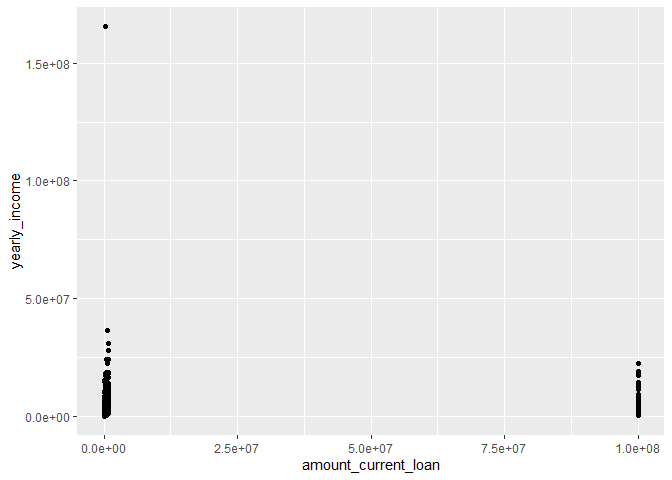
\includegraphics{report_files/figure-latex/Current Loan Amount and Yearly Income-1.pdf}

\hypertarget{second-plot}{%
\subsection{Second plot}\label{second-plot}}

In the plot below we can inspect the relationship between Monthly Debt
Amount and Years of Credit History.

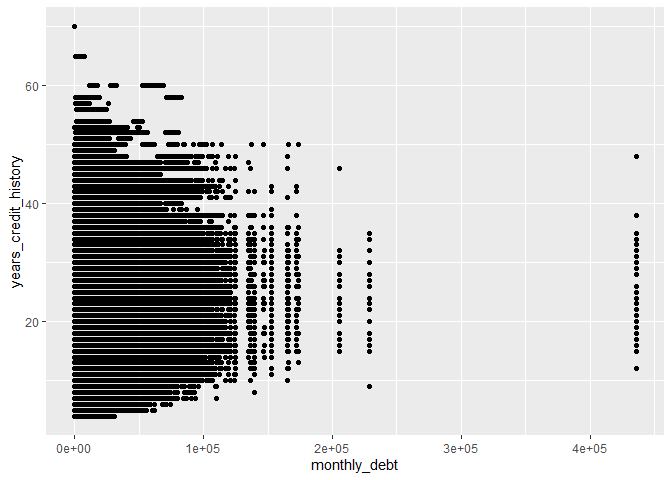
\includegraphics{report_files/figure-latex/Monthly Debt Amount and Years of Credit History-1.pdf}

\end{document}
